\documentclass{beamer}
\DeclareFontShape{OT1}{cmss}{b}{n}{<->ssub * cmss/bx/n}{} 
\usetheme{default}
\usepackage{amsmath}
\usepackage{amsfonts}
\usepackage{mathbbol}
\usepackage{xcolor} % before tikz or tkz-euclide if necessary
\usepackage{tkz-euclide} % no need to load TikZ
\usepackage{multirow}
\usepackage{bm}


\usepackage[
backend=biber,
style=authoryear-icomp,
sortlocale=de_DE,
natbib=true,
url=false, 
doi=true,
eprint=false
]{biblatex}
\addbibresource{../../Bibliography/main_ML.bib}

\titlegraphic{
\includegraphics[width=2cm]{../../Figures/UAMS_RGB.png}
}

\title{Statistical Machine Learning\\ Manifold Learning}
\author{Horacio G\'omez-Acevedo\\ Department of Biomedical Informatics}
\begin{document}
	\begin{frame}[plain]
		\maketitle
	\end{frame}
\begin{frame}{Linear Models}
	Popular methods of data analysis make the assumption that the data lies on a linear $k$-dimensional subspace of $\mathbb{R}^n$ where $k< n$. 
	
	The general problem reduces to search for a linear transformation $\theta \colon \mathbb{R}^n \to \mathbb{R}^k$ such that $\{\theta(x_i)\}$ retains something about the structure of $\{x_i\}$. 
	
	Linear models are ubiquitous in sciences, but the assumption of linearity is often unrealistic. One alternative, is to consider that the data has been sampled from a (compact Riemannian) \textbf{manifold} ${\cal M}\subset \mathbb{R}^n$ of much lower dimension than $n$. 

\end{frame}

\begin{frame}{What is a manifold?}
	Roughly speaking, a manifold (of dimension 2) is a surface that locally behaves as a regular space in $\mathbb{R}^2$. In geometry, we refer to local properties as intrinsic. 
\begin{figure}[h]
	\centering
	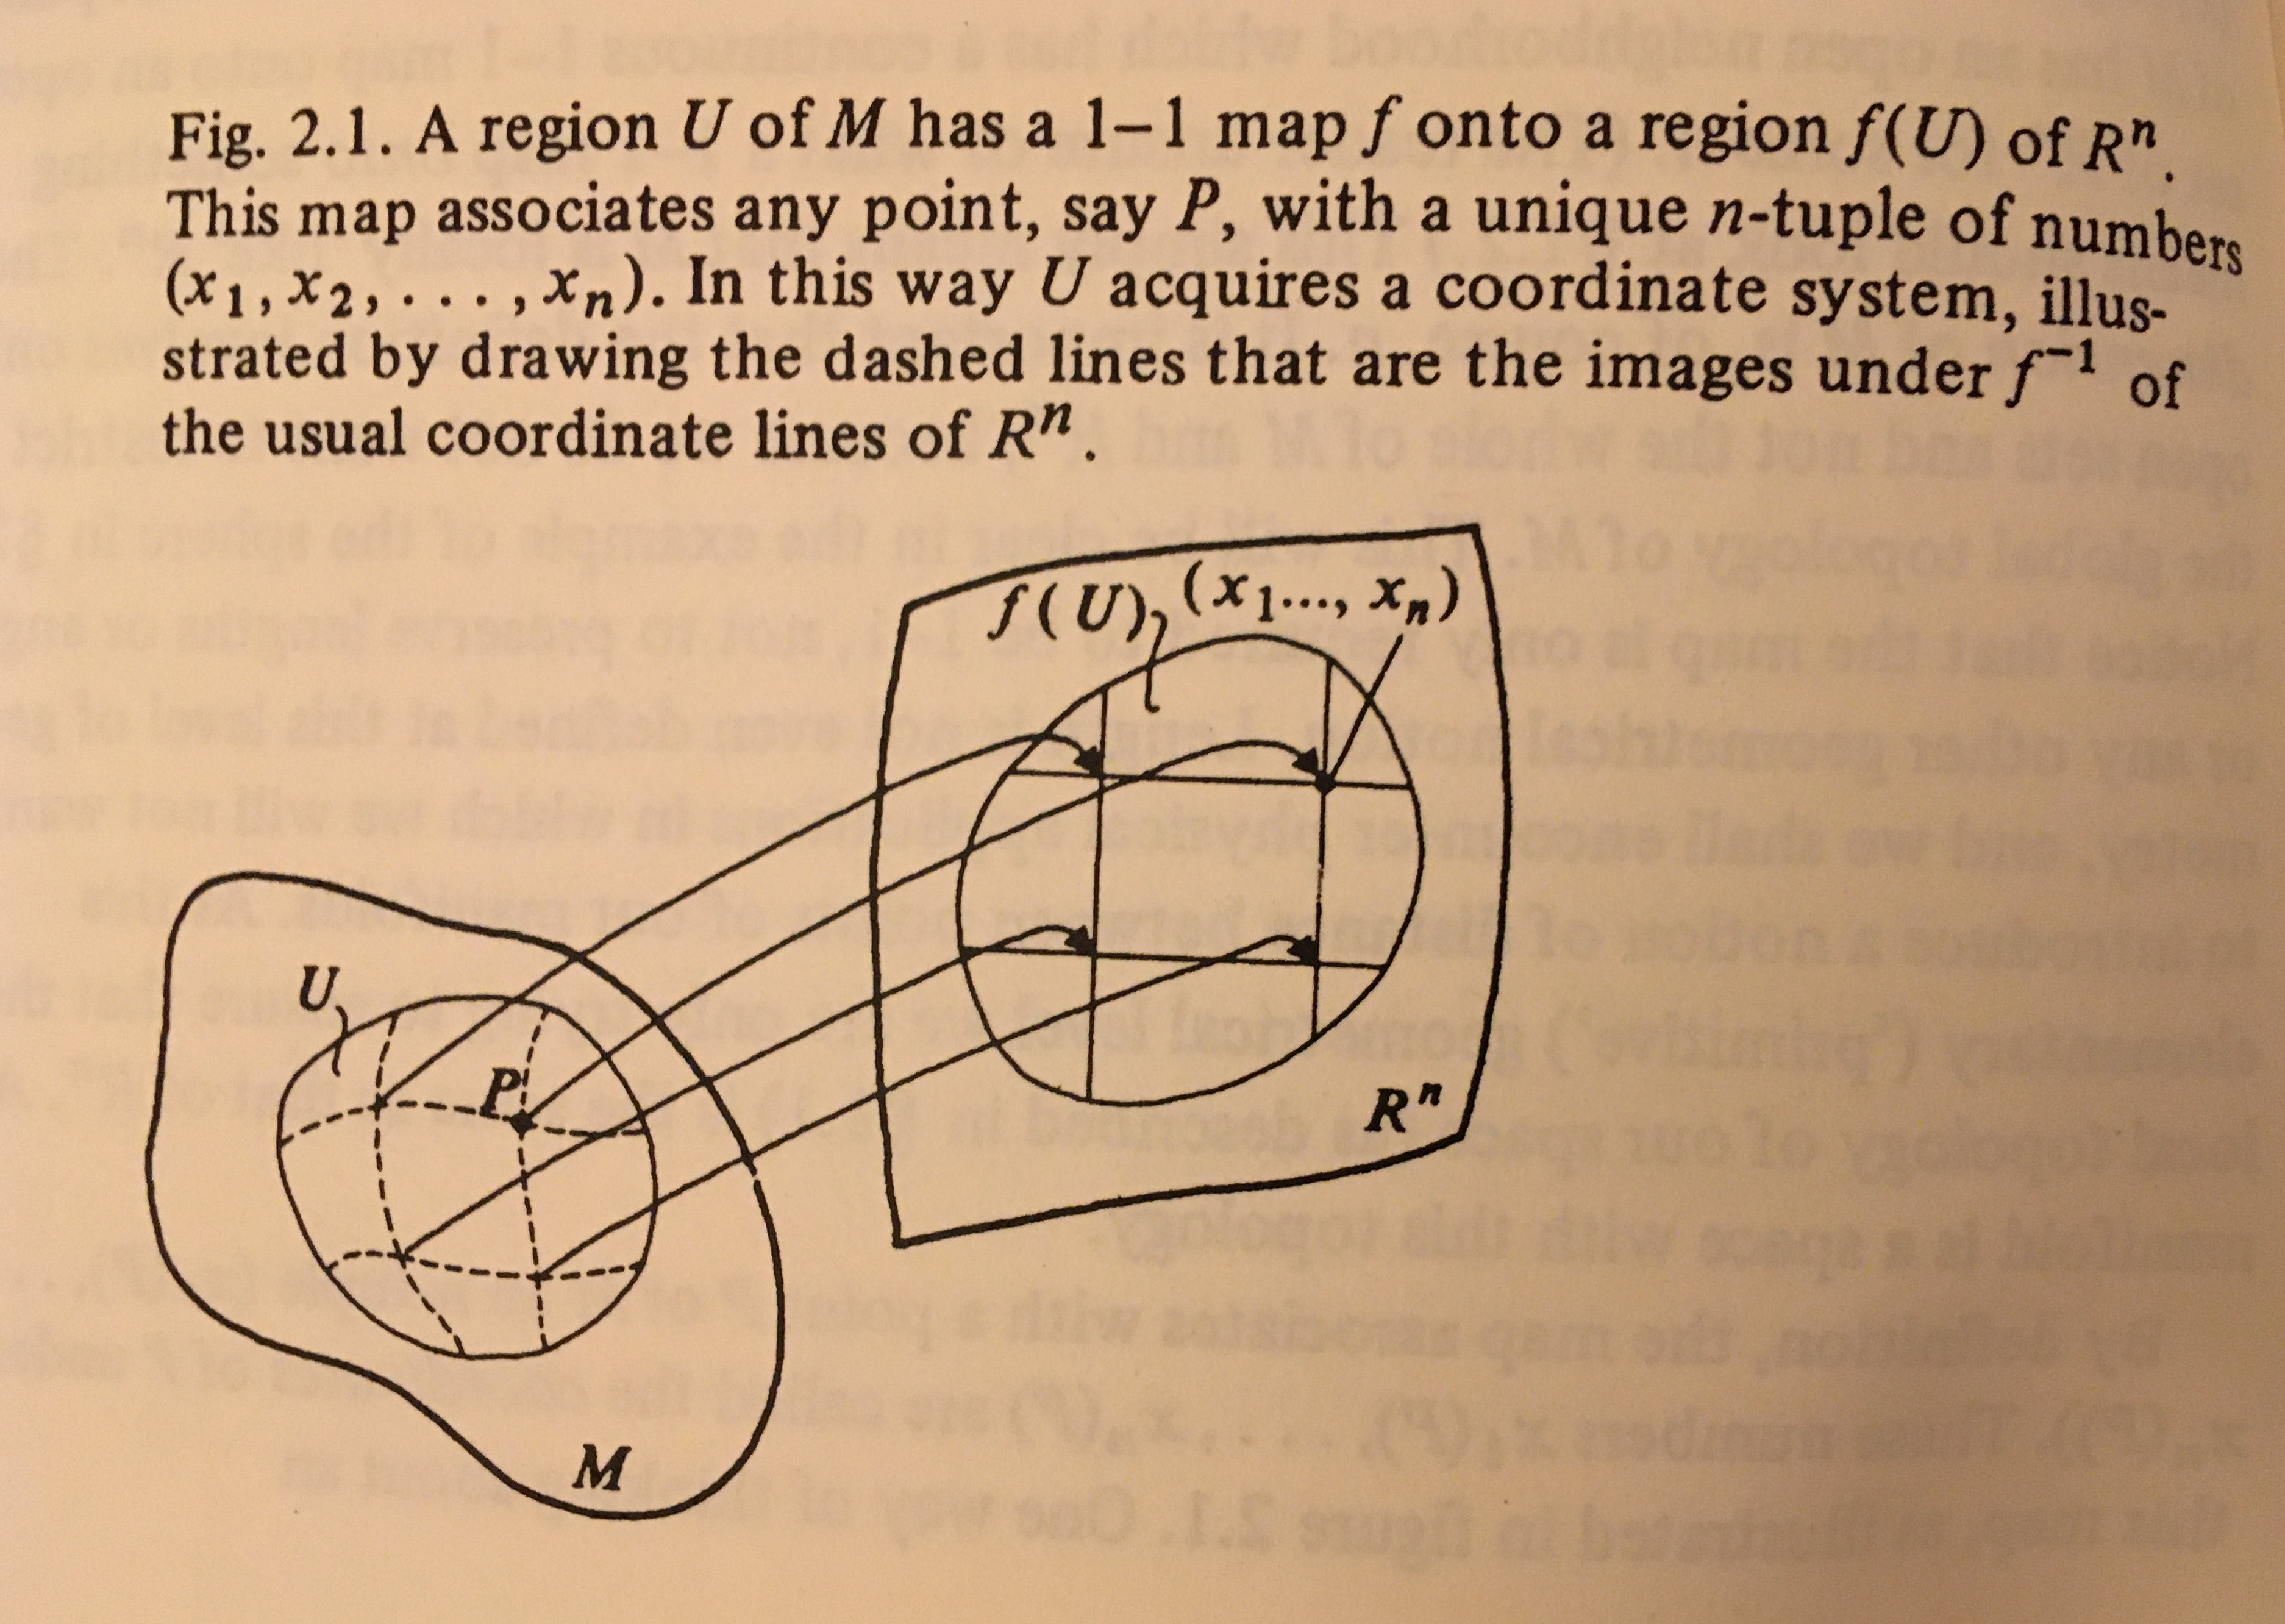
\includegraphics[width=7cm]{../../Figures/fig_manifold.jpg}
\end{figure}	
		
\end{frame}

\begin{frame}{The Sphere as a manifold}
	Another typical example is the sphere (often called $S^2$).
	
\begin{figure}[h]
	\centering
	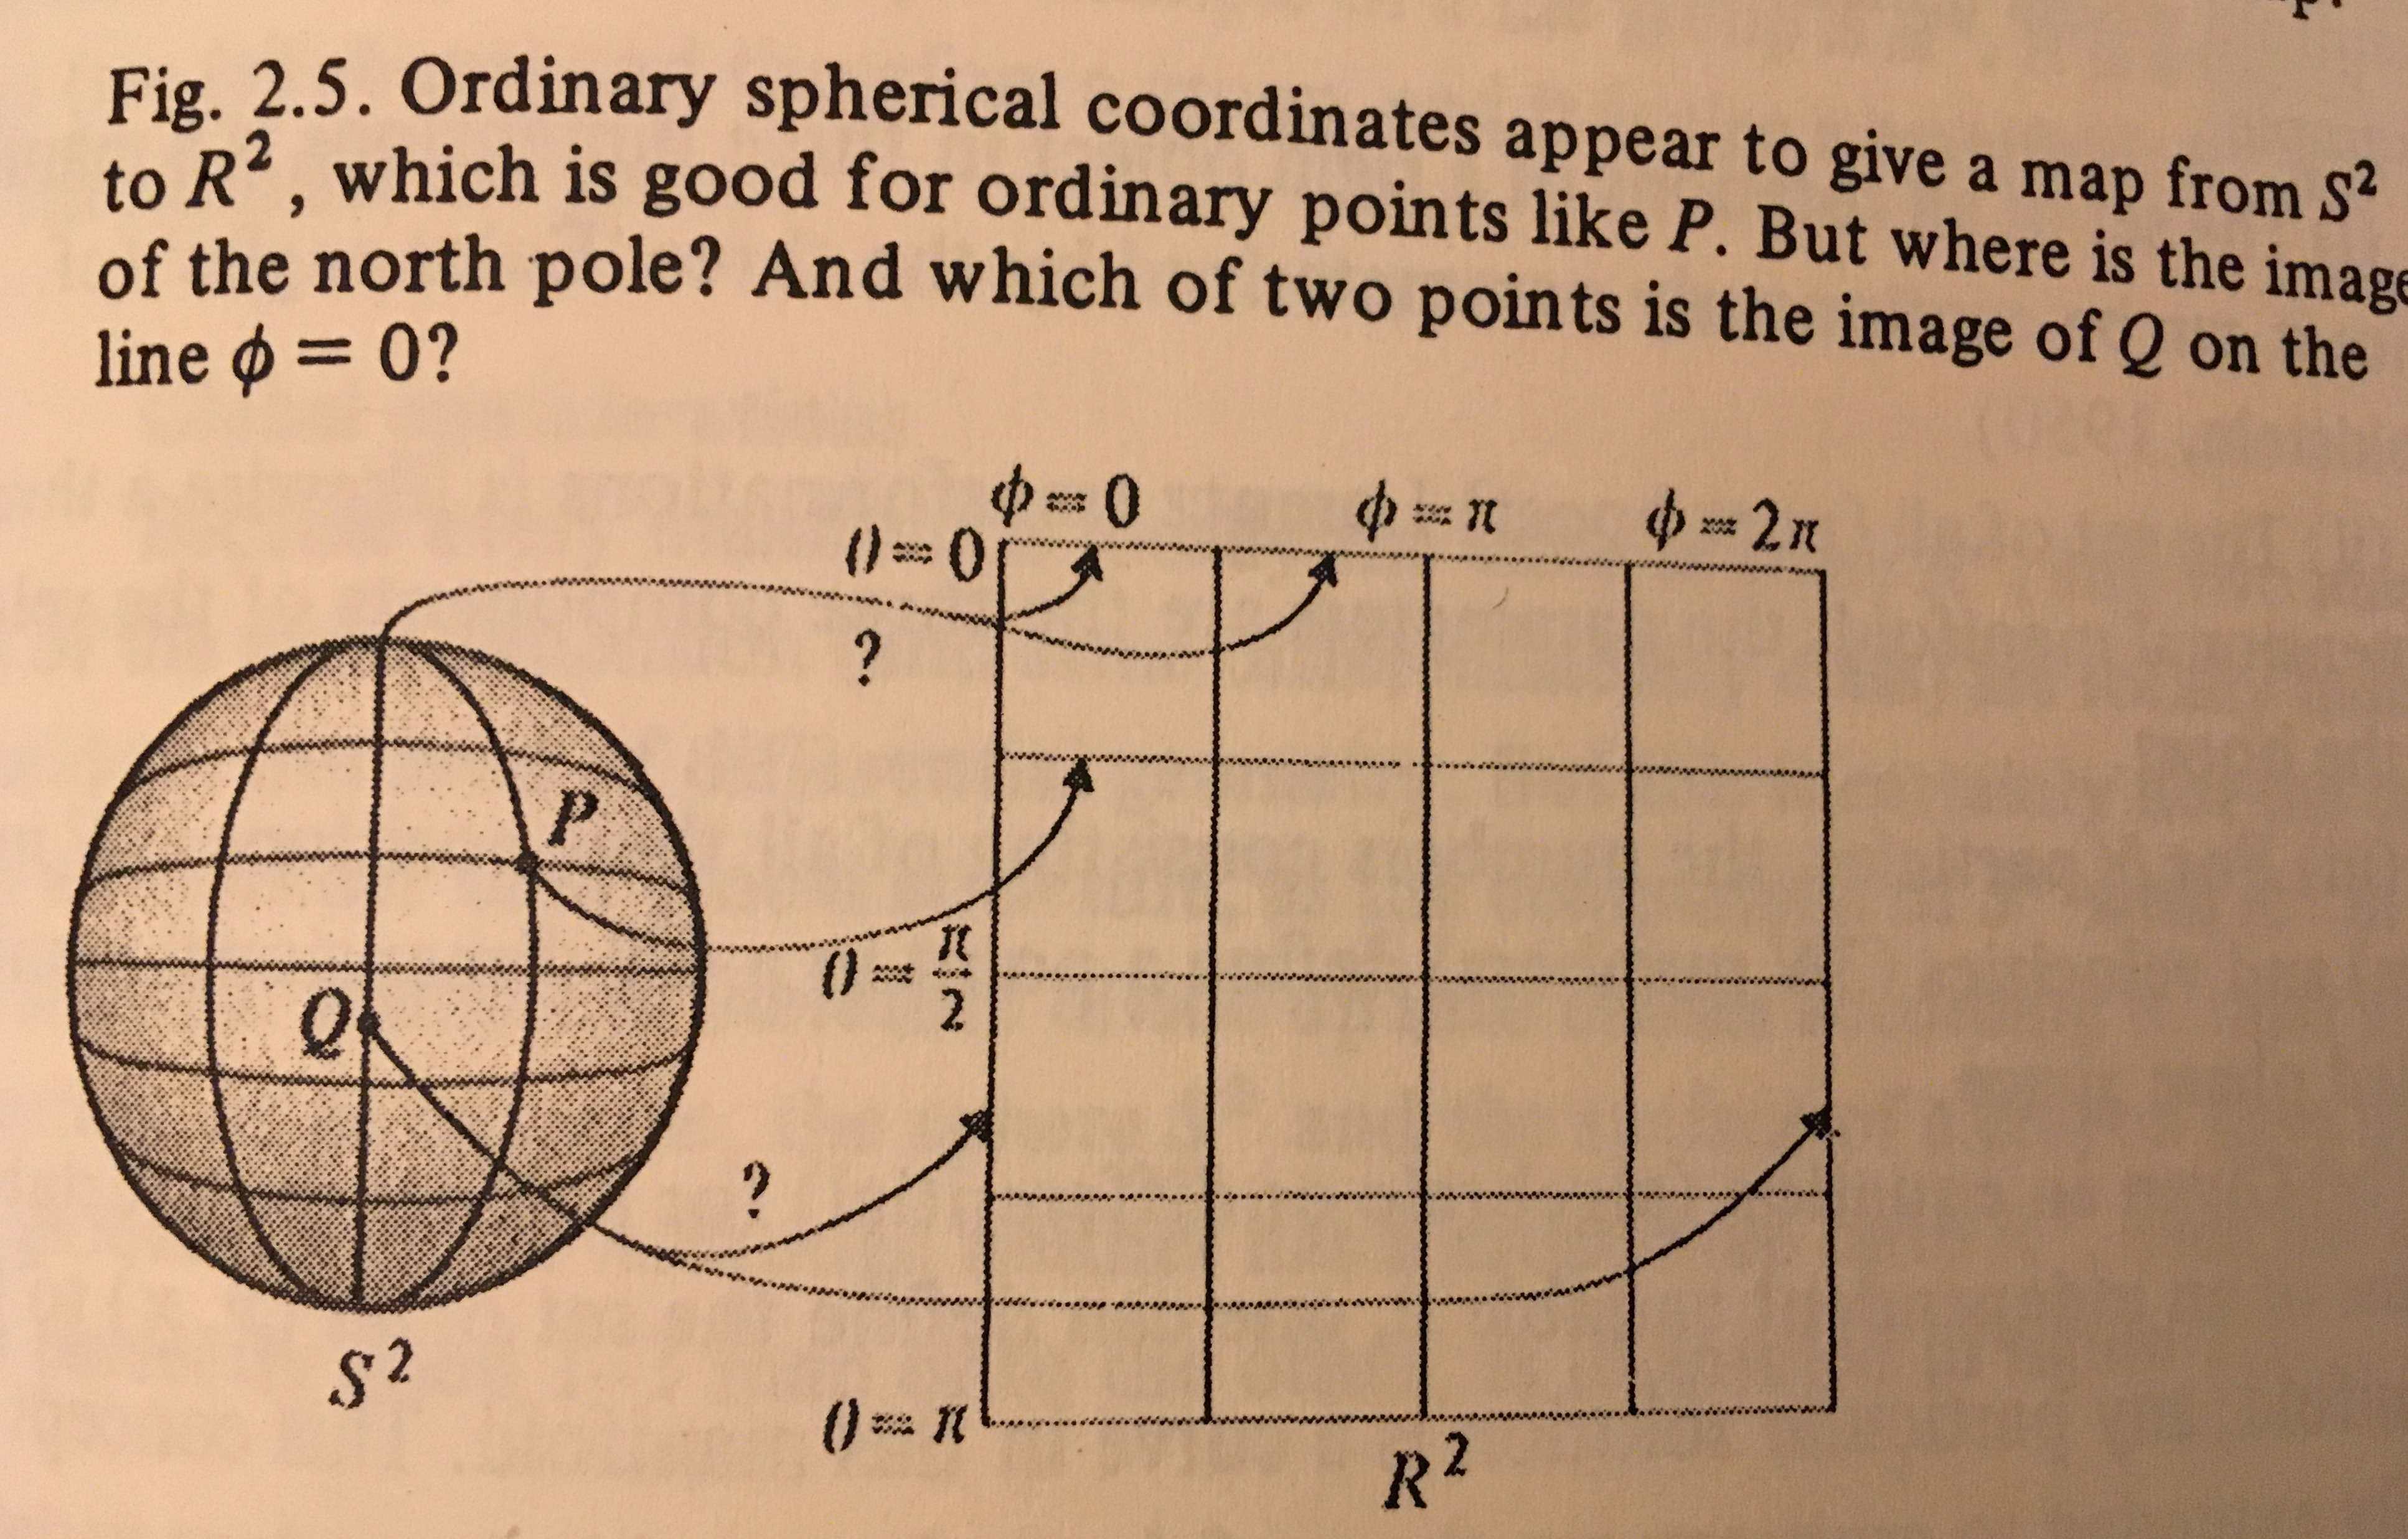
\includegraphics[width=7cm]{../../Figures/fig_manifold_sphere.jpg}
\end{figure}	
Intuitively, we cannot cover the whole sphere (in a unique way) with only one sheet. The north and south poles are a problem. 

\end{frame}

\begin{frame}{Sphere as a patch work}
	Instead, we use several overlapping sheets 
\begin{figure}[h]
	\centering
	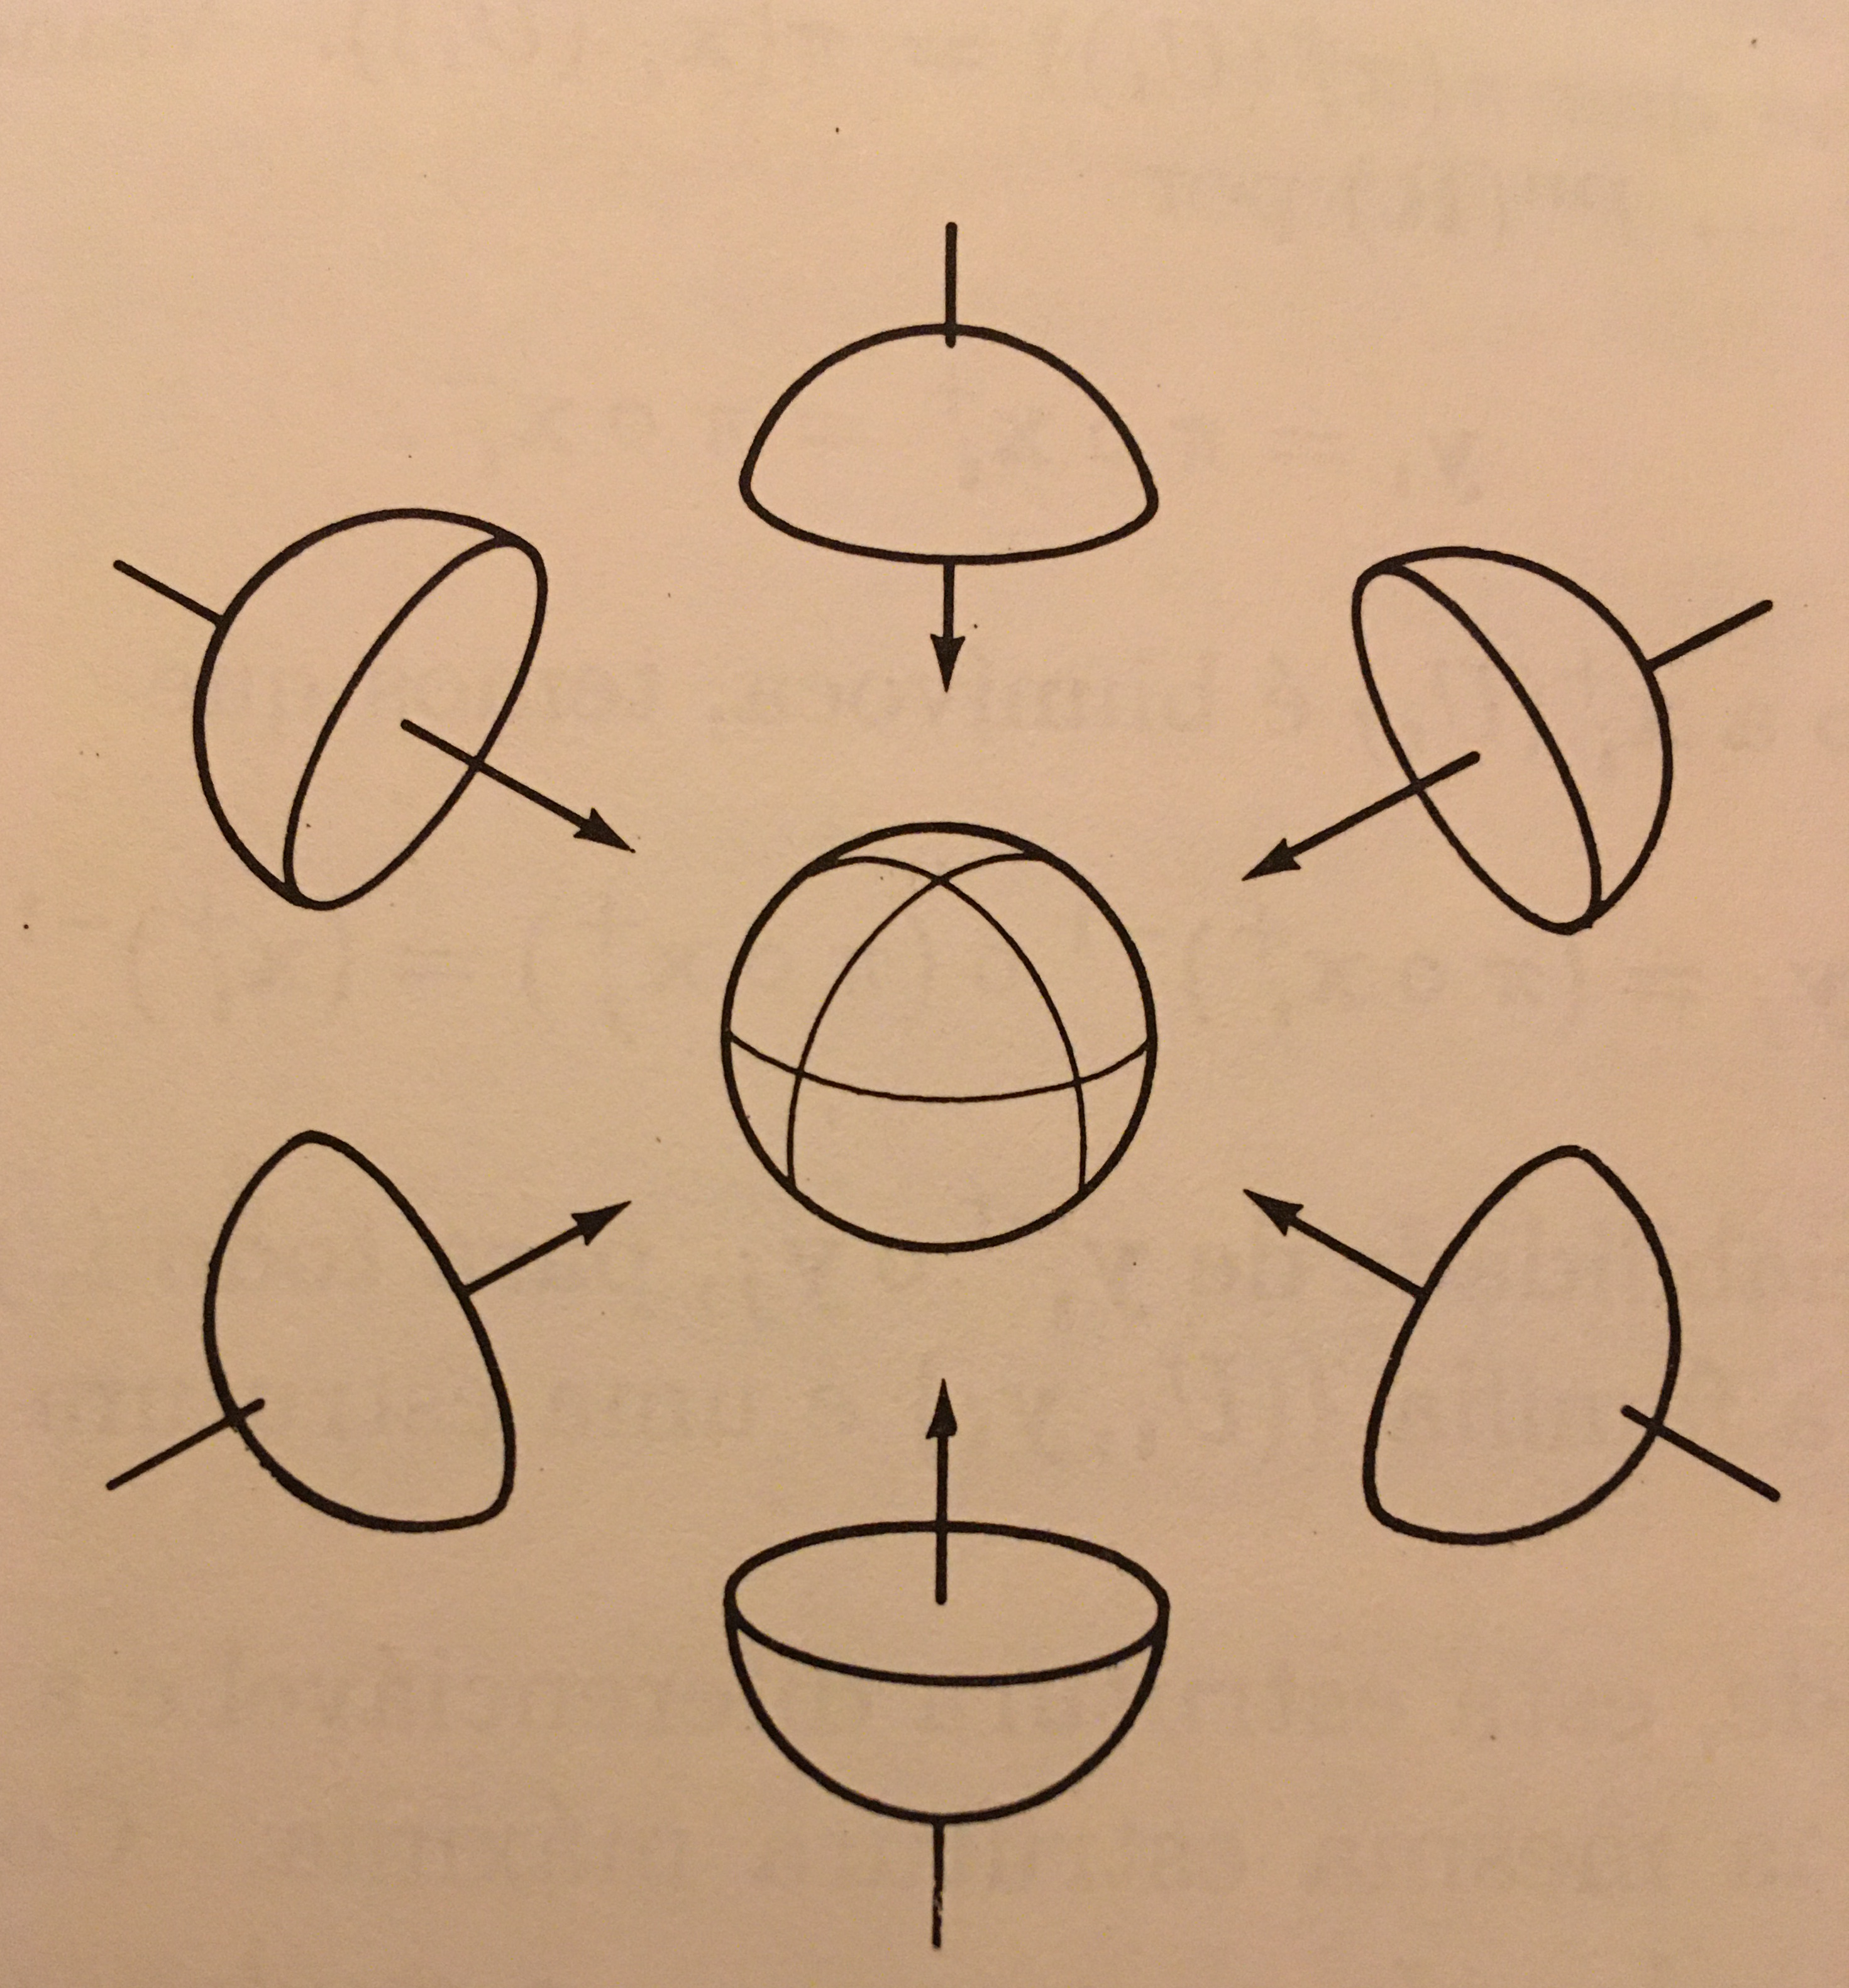
\includegraphics[width=6cm]{../../Figures/fig_manifold_sphere_2.jpg}
\end{figure}		
	
	
\end{frame}

\begin{frame}{Manifold Learning }
	
	Loosely speaking, the basic idea of most manifold learning techniques is to take the $k$-nearest neighbors of a point $x$ and use the vectors specified by the line segments from $x$ to its neighbors as an approximation for the tangent plane at $x$. 
	
	Global optimization then sews these local approximations together to produce a low-dimensional representation of the data. 
	
\begin{center}
\textbf{Manifold learning is also known as dimensionality reduction.} 
\end{center}
\end{frame}


\begin{frame}{PCA}
	In a general setup, we can think that we have $m$ vectors in $\mathbb{R}^n$, namely $\{x_1, \ldots, x_m\}$. We try to find the "optimal" linear projection $\theta \colon \mathbb{R}^n \to \mathbb{R}^k$ where $k \ll n$ (meaning $k$ much lower than $n$)
	\begin{enumerate}
	\item $\tilde{x_j} = x_j -\mu$ where $\mu= \frac{1}{m} \sum x_j$
	\item We find the variance-covariance matrix 
	\begin{equation*}
		C=\frac{1}{m} \sum_{j=1}^m \tilde{x_j} \tilde{x_j}^t
	\end{equation*}
	\item We compute the top $k$-eigenvectors $\{v_1, \ldots, v_k\}$ of $C$.
	\item These eigenvectors span a hyperplane (subspace) of $\mathbb{R}^n$. The projection $\theta \colon \mathbb{R}^n \to \mathbb{R}^k$ is precisely the orthogonal projection onto this plane followed by a choice of identification of the plane with $\mathbb{R}^k$.
	\item We can think $\theta$ as 
	\begin{equation*}
		y_j= \theta(\tilde{x_j})+ \mu
	\end{equation*}
	
	\end{enumerate}


\end{frame}

\begin{frame}{PCA cont}
	The process chooses the basis which maximizes the variance captured by the representation; the eigenvector $v_1$ with the largest eigenvalue is the single direction that captures the maximal amount of information about the variance; the plane spanned by $\{v_1,v_2\}$ is the plane with the most variance, etc.
	
	Another characterization of PCA is to find a projection that minimizes the error function
	\begin{equation*}
		E= \sum_{j=1}^m \| x_j -y_j \|^2, 
	\end{equation*}
	where $\| \cdot \|$ denotes some distance. For PCA this means that it produces the points $\{y_i\}$ that minimize the reconstruction error among all projections onto a $k$ dimensional subspace. 
\end{frame}

\begin{frame}{Multidimensional scaling (MDS)}

In this methodology, we search for a mapping $\theta \colon \mathbb{R}^n \to \mathbb{R}^k$ that minimizes
\begin{equation*}
	{\cal E}= \sum_{x_i,x_j} ( \|x_i -x_j \| - \|\theta(x_i)-\theta(x_j)\|)^2
\end{equation*}
The procedure is as follows. 
\begin{enumerate}
	\item Consider the matrix of the original distances $D=(D_{ij})$ where $D_{ij}= \|x_i -x_j\|$. 
	\item Set $H= I_n - \frac{1}{n} \mathbb{1} \cdot \mathbb{1}^t$, where $\mathbb{1}= (1,1, \ldots, 1)$. Set $Z= -\frac{1}{2} H D H$.
	\item The function that minimizes $\cal E$ is then given by finding the eigenvectors $v_j$ of $Z$. The $\theta(x_j)$ is specified by normalizing so that $\|v_j\|^2=\lambda_j$.
\end{enumerate}
\end{frame}

\begin{frame}{Manifold Learning Main Ideas}
	Suppose that we are given data points $\{x_1, \ldots, x_m\}$ in $\mathbb{R}^n$. We will assume that there is a function (embedding) $\gamma \colon {\cal M} \to \mathbb{R}^n$. 
	
	Keep in mind that \textit{distances} in manifolds can be different
\begin{figure}[h]
	\centering
	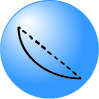
\includegraphics[width=3cm]{../../Figures/fig_geodesic.jpg}
\end{figure}
	The manifold structure can be reconstructed by considering the "short distances" as reliable indicators of the local (intrinsic) distances and ignoring the "long distances".
	

\end{frame}

\begin{frame}{What we have learned?	}
	\begin{itemize}
		\item The power of resampling methods for estimation of parameters.
		\item Bootstrap is considered one of the most powerful statistical techniques for estimation. 
		\item Methods for subset selection of covariates in a regression setting.
		\item We explore the forward and backward selection.
	\end{itemize}
\end{frame}

\begin{frame}{Isomap}
	Isomap applies MDS to an empirical approximation of the intrinsic metric.
	The procedure goes as follows. We fix a scale parameter $\varepsilon$ and a target dimension parameter $k$.
	
	\begin{enumerate}
		\item Form the weighted graph $G$ with
		\begin{itemize}
			\item vertices the points $\{x_i\}$, and
			\item edges $(i,j)$ with weights given by $w_{ij}=\| x_i -x_j\|$ when $\|x_i -x_j\| \le \varepsilon$.
		\end{itemize}
		\item We form a new space $X'$ with points $\{x_i\}$ but distances given by the graph metric on $G$.  Meaning that the distances between two edges is given by the shortest path in the graph.
		\item Use MDS to embed this space into $\mathbb{R}^k$ producing points $y_i = \theta(x_i)$
	\end{enumerate}
\end{frame}


\begin{frame}{References}
	Some of the pictures are from \citep{docarmoriemann}, and \citep{schutz}, and \citep{geron2}. Main reference for manifold learning \citep{rabadan}.
	\printbibliography 	
	
	I have used some of the graphs by hacking TiKz code from StakExchange, Inkscape for more aesthetic plots and other old tricks of \TeX
	
\end{frame}


	
\end{document}
